\section{Constructing the outcome: successor linkage}

\subsection{Why this step exists}

Survival analysis needs two numbers per awarded procurement episode: a delay and an event indicator. The BOAMP supplies neither. This section builds both, and measures the quality of that construction --- because an error here is corrected nowhere downstream.

\subsection{Candidate generation}

For each \textbf{anchor} \(i\) (an awarded cohort episode with origin \(u_i\)), a later episode \(j\) with origin \(v_j\) is exposed for comparison if and only if:

\begin{itemize}
\tightlist
\item
  buyer identifiers are compatible --- same buyer key or same normalised name, with two different validated SIRENs disqualifying;
\item
  and the chronology satisfies
  \[u_i + 90\ \text{days} \le v_j \le u_i + 2{,}920\ \text{days}.\]
\end{itemize}

The 90-day to 8-year window is an \textbf{operational search range}, not an assumed contract duration. Git and notebook history place the 90-day floor in the candidate-generation notebook committed on 11 August 2026, before the final pipeline was frozen. It responded to a clear concurrent-procurement pathology: without a floor, \texttt{132} of the \texttt{628} links then accepted fell within three months of award, and every link for a 2025 award sat under twelve months, with a median of 1.7. The same design check also used the full reviewed successor set: the shortest of the 23 reviewed gaps was \textbf{139 days}, so the floor excluded none of them. Candidate generation was therefore informed by broader reference diagnostics, including the designated locked stratum; it was not evaluated as an untouched component. The eight-year ceiling likewise excludes no reviewed successor.

The result is \textbf{763,417 pairs} covering \textbf{3,520 of the 3,800 anchors}. The 280 anchors with no candidate at all stay in the analysis as censored exposure: their status is decided by blocking, not by the acceptance bar.

\textbf{No hard CPV filter, and the argument is empirical.} Requiring the successor to share the anchor's CPV division would be tempting. The reference forbids it: of the 23 reviewed successors, \textbf{9 (39.1 \%) cross a division}. Hard blocking would destroy them and cut the attainable recall ceiling from 0.913 to 0.609. The literature points the same way: CPV assignment is documented as error-prone even for experts \citep{siciliani2023}. CPV is therefore used as continuity evidence, never as a hard constraint.

\subsection{Four methods on the same pairs}

\begingroup\small
\begin{longtable}[]{@{}
  >{\raggedright\arraybackslash}p{(\columnwidth - 4\tabcolsep) * \real{0.3333}}
  >{\raggedright\arraybackslash}p{(\columnwidth - 4\tabcolsep) * \real{0.3333}}
  >{\raggedright\arraybackslash}p{(\columnwidth - 4\tabcolsep) * \real{0.3333}}@{}}
\toprule\noalign{}
\begin{minipage}[b]{\linewidth}\raggedright
M.
\end{minipage} & \begin{minipage}[b]{\linewidth}\raggedright
Role
\end{minipage} & \begin{minipage}[b]{\linewidth}\raggedright
Principle
\end{minipage} \\
\midrule\noalign{}
\endhead
\bottomrule\noalign{}
\endlastfoot
\texttt{M\_A\_deterministic} & Conservative comparator & Requires buyer, CPV and a minimum text-similarity floor \\
\texttt{M\_B\_text\_ranking} & \textbf{Primary method} & Takes the highest TF-IDF cosine candidate and accepts it above the threshold \\
\texttt{M\_C\_weighted\_gated} & High-recall comparator & Weighted score, buyer 0.50 / text 0.25 / CPV 0.20 / time 0.05, renormalised over observed evidence \\
\texttt{M\_D\_fellegi\_sunter} & Probabilistic comparator & Match / non-match likelihood ratios \citep{fellegi1969} \\
\end{longtable}
\endgroup

The primary decision rule is
\[\hat{j}_i = \arg\max_{j \in J_i} T_{ij}, \qquad Y_i = \mathbf{1}\!\left(T_{i\hat{j}_i} \ge 0.70\right),\]
where \(T_{ij}\) is the maximum of a word-level and a character-level TF-IDF cosine similarity. \textbf{At most one successor per anchor}; otherwise the method abstains.

One implementation detail has consequences analysed in \S~5.7: the vectoriser is fitted \emph{per anchor block}. That choice has a reason --- the IDF weights become local to the buyer's own vocabulary, which stops the administrative boilerplate common to all of a buyer's notices from dominating the similarity --- and it has a cost: the score becomes block-relative, a fixed 0.70 does not mean quite the same thing for every anchor, and the maximum over a larger block is mechanically higher. \S~5.7d measures that cost rather than assuming it negligible.

\subsection{Operating-point chronology and validation status}

The 0.70 threshold follows a precision-first principle: a false link fabricates both an event and its date, whereas a missed link does not fabricate an event. The project history nevertheless does \textbf{not} support calling its final reference result fully held out. An earlier committed linkage script records that the \texttt{M\_B @ 0.70} policy drew on inspection of the designated locked split; candidate-generation diagnostics also used the full reviewed successor set. The operating point was subsequently frozen and never moved, so the current sweep is a transparent \textbf{internal validation and sensitivity display}, not an untouched external test of every pipeline decision. The 0.60 arm is retained to show the precision--recall trade rather than promoted post hoc.

The brief anticipated a linkage rate of 40-60 \%. The realised rate is \textbf{14.3 \%}. This is not a shortfall against a target: the brief's figure was treated as a planning assumption, never as an optimisation objective, and 14.3 \% is the arithmetic consequence of a precision-first rule combined with an event defined as \emph{observable in the BOAMP}.

\begin{figure}[htbp]
\centering
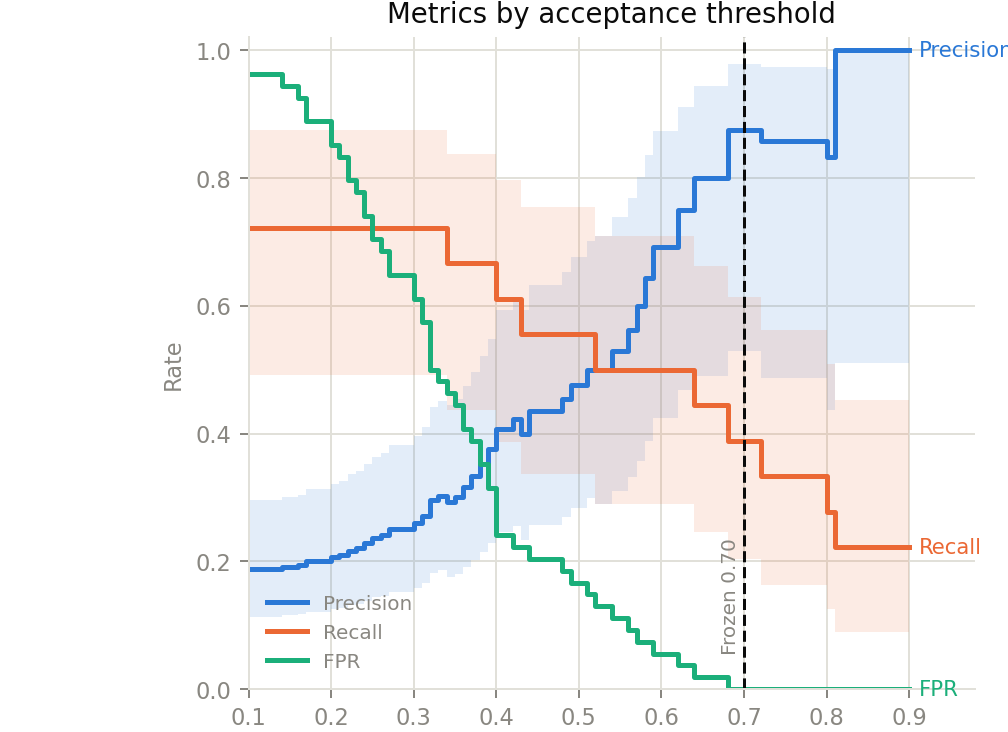
\includegraphics[width=0.78\linewidth]{figures/fig05_threshold_left_panel.png}
\caption{Precision, recall, false-positive rate and accepted-link volume as a function of the \texttt{M\_B} acceptance threshold on the reference stratum designated \texttt{LOCKED\_TEST}. The retained 0.70 operating point is marked. Project history shows that this evidence informed the final policy, so the panel is an internal-validation display rather than an untouched holdout. Shaded bands are 95\,\% Wilson intervals and every riser is one anchor changing decision, on 72 anchors of which 18 have a reviewed successor. The full three-panel version is Figure~\ref{fig:appc-tradeoff} in Annex C.}
\label{fig:threshold}
\end{figure}


\subsection{The regional reference, and what it is worth}

The evaluation strategy follows the three-part scheme recommended for linked data \citep{harron2017}: score the algorithm on a reference subset, compare linked with unlinked records, and test whether conclusions survive changes to the linkage procedure. Evaluation rests on a stratified review of \textbf{120 Grand Ouest anchors}, carried out on 11 August 2026 against the real BOAMP notices and their official URLs, \textbf{before the linkage methods in this project existed}. 112 anchors re-resolve onto exactly one episode and 88 are usable; the pilot (16 anchors) / locked (72 anchors) split is recorded in the reference file itself and is not post hoc.

Four limits bound its reach, and they belong in the body of the report rather than in a footnote:

\begin{enumerate}
\def\labelenumi{\arabic{enumi}.}
\tightlist
\item
  \textbf{The labels come from a single large-language-model research pass}, spot-checked by the project owner rather than verified anchor by anchor, and not judged by a specialist panel. They are independent of every method scored --- none existed at the time --- but they are not human ground truth.
\item
  \textbf{The per-anchor evidence trail was not recorded}: the sources behind a given decision cannot be reconstructed.
\item
  \textbf{Negatives are corpus-relative}: roughly 25 candidates per anchor were considered, not the full pool. A negative means ``no successor identified among those examined''.
\item
  \textbf{Candidate-surfacing independence does not hold.} The rule that selected those \textasciitilde25 candidates (from pools of up to 3,258) is recorded nowhere, and all 16 retrievable locked-split successors rank within the top thirteen by the very text score being evaluated. Consequently \textbf{recall and the 0.913 ceiling are not fully independent of the score they bound}. Precision is unaffected: a false positive is a false positive however the list was assembled.
\end{enumerate}

\subsection{Internal-validation results on the designated locked stratum}

Two accountings coexist and do not answer the same question. \emph{Anchor-level} accounting asks whether the system detected that a successor exists. \emph{Exact-successor} accounting, which is stricter, asks whether it named the right one; a wrong successor on a positive anchor then counts as one false positive \textbf{and} one false negative. The project's headline figures are the latter.

\begingroup\footnotesize
\begin{longtable}[]{@{}
  >{\raggedright\arraybackslash}p{(\columnwidth - 18\tabcolsep) * \real{0.0811}}
  >{\raggedright\arraybackslash}p{(\columnwidth - 18\tabcolsep) * \real{0.0811}}
  >{\raggedleft\arraybackslash}p{(\columnwidth - 18\tabcolsep) * \real{0.1081}}
  >{\raggedleft\arraybackslash}p{(\columnwidth - 18\tabcolsep) * \real{0.1081}}
  >{\raggedleft\arraybackslash}p{(\columnwidth - 18\tabcolsep) * \real{0.1081}}
  >{\raggedleft\arraybackslash}p{(\columnwidth - 18\tabcolsep) * \real{0.1081}}
  >{\raggedleft\arraybackslash}p{(\columnwidth - 18\tabcolsep) * \real{0.1081}}
  >{\raggedright\arraybackslash}p{(\columnwidth - 18\tabcolsep) * \real{0.0811}}
  >{\raggedleft\arraybackslash}p{(\columnwidth - 18\tabcolsep) * \real{0.1081}}
  >{\raggedleft\arraybackslash}p{(\columnwidth - 18\tabcolsep) * \real{0.1081}}@{}}
\toprule\noalign{}
\begin{minipage}[b]{\linewidth}\raggedright
M.
\end{minipage} & \begin{minipage}[b]{\linewidth}\raggedright
Thr.
\end{minipage} & \begin{minipage}[b]{\linewidth}\raggedleft
TP
\end{minipage} & \begin{minipage}[b]{\linewidth}\raggedleft
FP
\end{minipage} & \begin{minipage}[b]{\linewidth}\raggedleft
FN
\end{minipage} & \begin{minipage}[b]{\linewidth}\raggedleft
TN
\end{minipage} & \begin{minipage}[b]{\linewidth}\raggedleft
Precision
\end{minipage} & \begin{minipage}[b]{\linewidth}\raggedright
95 \% CI
\end{minipage} & \begin{minipage}[b]{\linewidth}\raggedleft
Recall
\end{minipage} & \begin{minipage}[b]{\linewidth}\raggedleft
FPR
\end{minipage} \\
\midrule\noalign{}
\endhead
\bottomrule\noalign{}
\endlastfoot
\texttt{M\_A} & n/a & 8 & 7 & 10 & 47 & 0.533 & 0.301-0.752 & 0.444 & 0.130 \\
\textbf{\texttt{M\_B}} & \textbf{0.70} & \textbf{7} & \textbf{1} & \textbf{11} & \textbf{54} & \textbf{0.875} & \textbf{0.529-0.978} & \textbf{0.389} & \textbf{0.000} \\
\texttt{M\_C} & 0.70 & 12 & 11 & 6 & 44 & 0.522 & 0.330-0.708 & 0.667 & 0.185 \\
\texttt{M\_D} & 0.65 & 1 & 4 & 17 & 53 & 0.200 & 0.036-0.625 & 0.056 & 0.018 \\
\end{longtable}
\endgroup

Three readings, in order of importance.

\textbf{The intervals overlap heavily.} A precision of 0.875 resting on \textbf{eight accepted links} has an interval running from ``coin flip'' to ``near perfect''. The figure must never be quoted without it, and this reference separates the methods only coarsely.

\textbf{Recall is capped before any scoring.} Candidate generation exposes only 21 of the 23 reviewed successors, a pairs completeness of 0.913 \citep{christen2007}; both unreachable cases are attributed to a named blocking condition --- one anchor never entered the cohort for want of a structured address, one buyer changed legal form from CCAS to CIAS with no shared SIREN. No unexplained case, which is what distinguishes an owned ceiling from an implementation defect.

\textbf{The precision-recall trade is deliberate.} \texttt{M\_C} buys recall (0.667) at half the precision (0.522). For survival analysis that is not a neutral exchange: its 11 false positives would introduce eleven events that never happened, with eleven dates that never happened.

\subsection{Challenge review and linkage audit}

A blinded 60-pair sample was prepared (20 production-accepted links, 20 high-similarity structural negatives, 20 buyer-declared relationships), with a separate audit key and a pre-specified acceptance rule. The review that was carried out is \textbf{model-assisted, not independent-human} --- its provenance is recorded explicitly in the repository. Of the 20 accepted links: 14 confirmed, 5 rejected, 1 uncertain, giving a precision of \textbf{0.700} on a conservative reading (95 \% CI {[}0.457; 0.881{]}), \textbf{below the 0.80 target} the project set itself.

The result is reported as it stands. It does not close the validation gate; it makes closing it necessary. Independent human review is the first recommendation in \S~9.F.

\subsection{What linkage produces}

\textbf{544 accepted links} over 3,800 anchors, an event rate of \textbf{14.32 \%}. CPV continuity: 351 of the 538 links with both divisions observed stay within one division (65.2 \%), comparable to the reviewed reference successors (14 of 23, 60.9 \%). 461 distinct successors for 544 links: 44 episodes are accepted by more than one anchor, the most reused by eleven --- a false-positive signature exploited in \S~5.7. Zero accepted links with conflicting validated SIRENs; zero municipality / inter-municipal mixes.
